\problemname{Mineskælv}
\illustration{.4}{img/Goodluck_Mine.jpg}{%
  \emph{Goodluck Mine, Passage} af Ashley Dace. 
  Licens CC BY-SA 2.0.}

\noindent
De helautonome mikrobryggerier, der er installeret i de forladte dværgminer af Moravia, bærer vitterligt vidnesbyrd om dværgfolkets opfindsomhed og håndværk!
Desværre rystes minerne sommetider af jordskælv, der fører til at de deraf forskudte rør og tragte spilder kostbar væske på gulvet.
Som den Ophøjede vogter for bryggerisikkerhed er det dit ansvar at slukke maskinerne i hver hal i tilfælde af et jordskælv.

Det tager tid at gå gennem tunnelerne,
så du vil uundgåeligt komme for sent til mange af maskinerne.
Dette kan ikke undgås, men du ønsker at minimere den samlede mængde af spildt væske.

\medskip
Dværgminerne består af $n$~haller forbundet af $n-1$~tunneler.
Hele systemet er forbundet, så det er muligt at komme fra hver hal til hver af de andre.
Det tager $1$~tidsenhed at passere en tunnel.
At slukke for en maskine og passere en hal tager ingen tid.
I hver hal gælder, at hvis maskinerne slukkes ved tidspunkt~$t$ efter jordskælvet, så spildes $t$~liter væske.
Der er præcis ét jordskælv, jordskælvet påvirker alle haller samtidigt, og du må ikke slukke for nogen maskiner inden jordskælvet.
Du kan starte i hvilken hal, du vil.



\subsection*{Eksempel}

I eksempel~$1$ ser minerne sådan her ud:

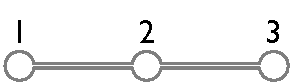
\includegraphics[width=.2\textwidth]{img/sample-1.pdf}

Hvis du begynder i hal~$2$ og besøger resten af hallene i rækkefølgen $2$, $1$, $2$, $3$, kan du slukke deres maskiner ved tid~$0$ (i hal $2$), tid~$1$ (i hal $1$) og tid~$3$ (i hal $3$).
Dette spilder sammenlagt $0+1+3=4$~liter væske.
Hvis du derimod starter i hal~$1$ og besøger hallerne i rækkefølgen $1$, $2$, $3$, så er den samlede mængde af spildt væske $0+1+2=3$~liter, hvilket er bedre.

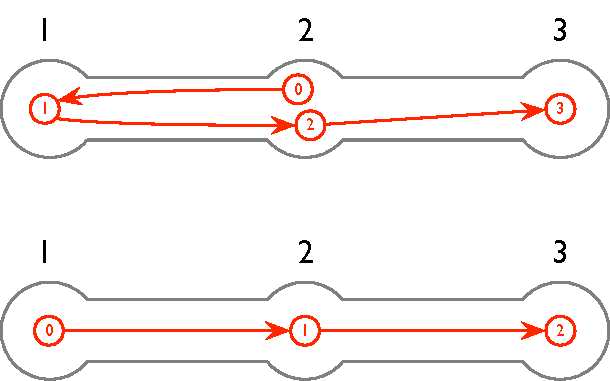
\includegraphics[width=.4\textwidth]{img/sample-1-ans.pdf}

\subsection*{Indlæsning}

Første linje af indlæsningen består af heltallet $n$, som angiver antallet af haller.
Vi antager, at hallerne er nummeret $1$, $\ldots$, $n$.

Hver af de næste $n-1$ linjer består af to heltal $u$ og $v$, adskilte af mellemrum, som opfylder
$1\leq u < v \leq n$ % constraint:hallnames
og betyder, at der er en tunnel mellem hal~$u$ og hal~$v$.

\subsection*{Udskrift}

Skriv et enkelt heltal: det mindste antal liter af spildt væske.

\subsection*{Begrænsninger og pointsætning}

Der gælder altid
$1\leq n\leq 10^5$. % constraint:n

Your solution will be tested on a set of test groups, each worth a number of points.
Each test group contains a set of test cases.
To get the points for a test group you need to solve all test cases in the test group.
Your final score will be the maximum score of a single submission.

\medskip
\begin{tabular}{lll}
  Gruppe & Points & Begrænsninger \\\hline
  $1$ & $18$ & ingen hal har mere end to tunneler\\
  $2$ & $19$ & højst en hal har mere end to tunneler\\
  $3$ & $20$ & $n\leq 10$\\
  $4$ & $21$ & $n\leq 1000$\\
  $5$ & $22$ & \emph{ingen yderligere begrænsninger}
\end{tabular}
